\section{Results}
\label{sec:results}

% =============================================================================
% Main-paper results figures. All plots are in pages/figures/ as PDFs.
% Tables with full numerical detail are in pages/appendix/results.tex.
% All values below are SIMULATED — replace with real numbers.
% =============================================================================

\subsection{GRPO Training Dynamics}
\label{sec:results_grpo}

\begin{figure*}[t]
    \centering
    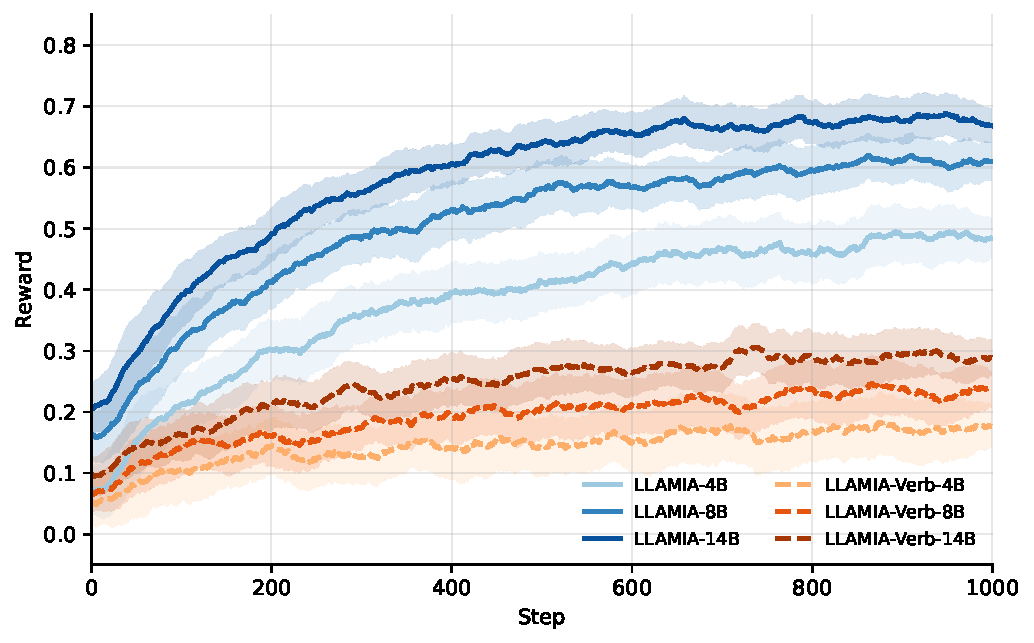
\includegraphics[width=\linewidth]{pages/figures/llamia_grpo_curves.pdf}
    \caption{\textbf{GRPO training reward: LLAMIA vs.\ LLAMIA-Verb.}
    Mean reward vs.\ training step at three model sizes (4B, 8B, 14B).
    Solid lines: LLAMIA (latent-state internalization).
    Dashed lines: LLAMIA-Verb (verbalized Lc0 tool call, same GRPO recipe).
    Shaded bands: running standard deviation.
    Internalization consistently reaches $2$--$3\times$ higher reward than
    verbalized tool use across all sizes, with the gap widening during training.
    }
    \label{fig:grpo_curves}
\end{figure*}

\begin{figure*}[t]
    \centering
    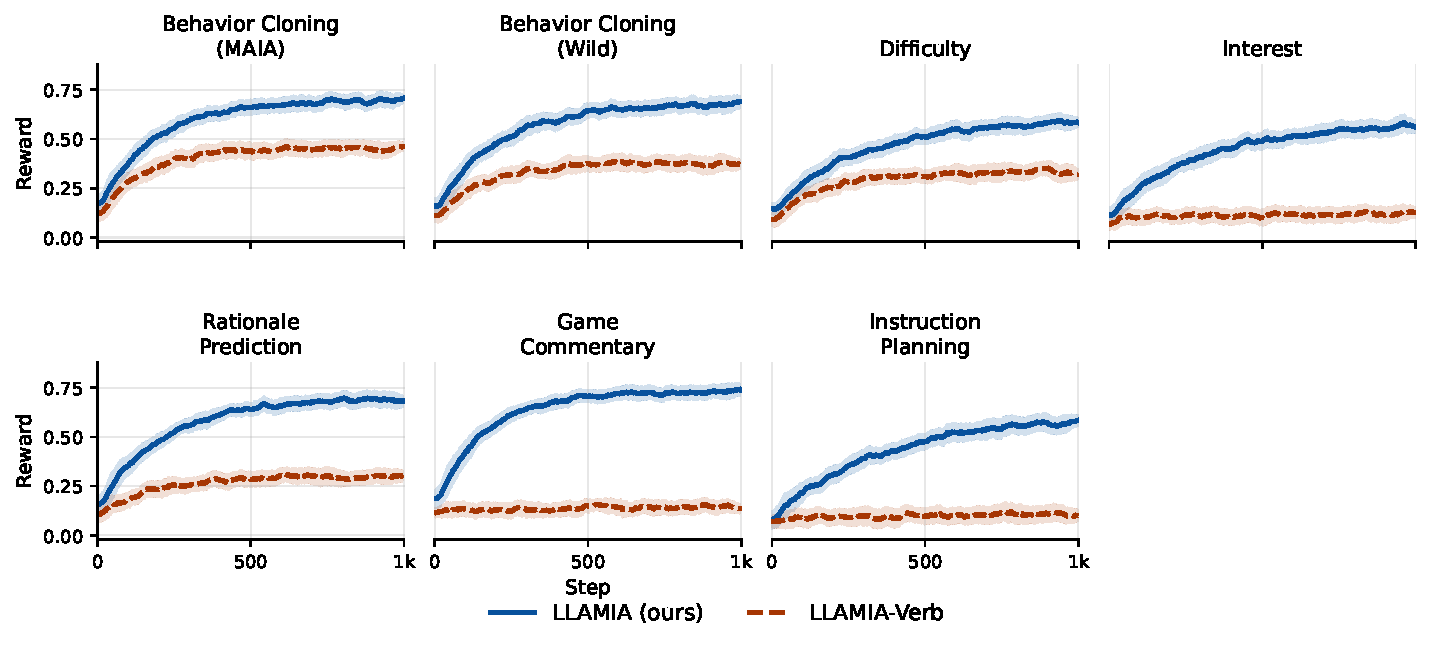
\includegraphics[width=\linewidth]{pages/figures/train_reward_curves.pdf}
    \caption{\textbf{Per-task train reward curves (LLAMIA vs.\ LLAMIA-Verb,
    4B/8B/14B).}
    Each panel shows one of six LLAMIA-Bench tasks (ICP shown separately
    as eval reward in Fig.~\ref{fig:icp_eval}).
    Solid lines: LLAMIA; dashed lines: LLAMIA-Verb; shade indicates
    model size (darker = larger).
    LLAMIA optimizes reward across all tasks and sizes.
    LLAMIA-Verb achieves partial signal on Behavior Cloning and Difficulty
    but stays flat on Interest, Rationale Prediction, and Game
    Commentary---tasks where the target signal is either
    non-verbalizable (Interest) or requires multi-step state tracking
    (Commentary).
    }
    \label{fig:train_reward_curves}
\end{figure*}

\subsection{LLAMIA-Bench Overview}
\label{sec:results_bench}

\begin{figure*}[t]
    \centering
    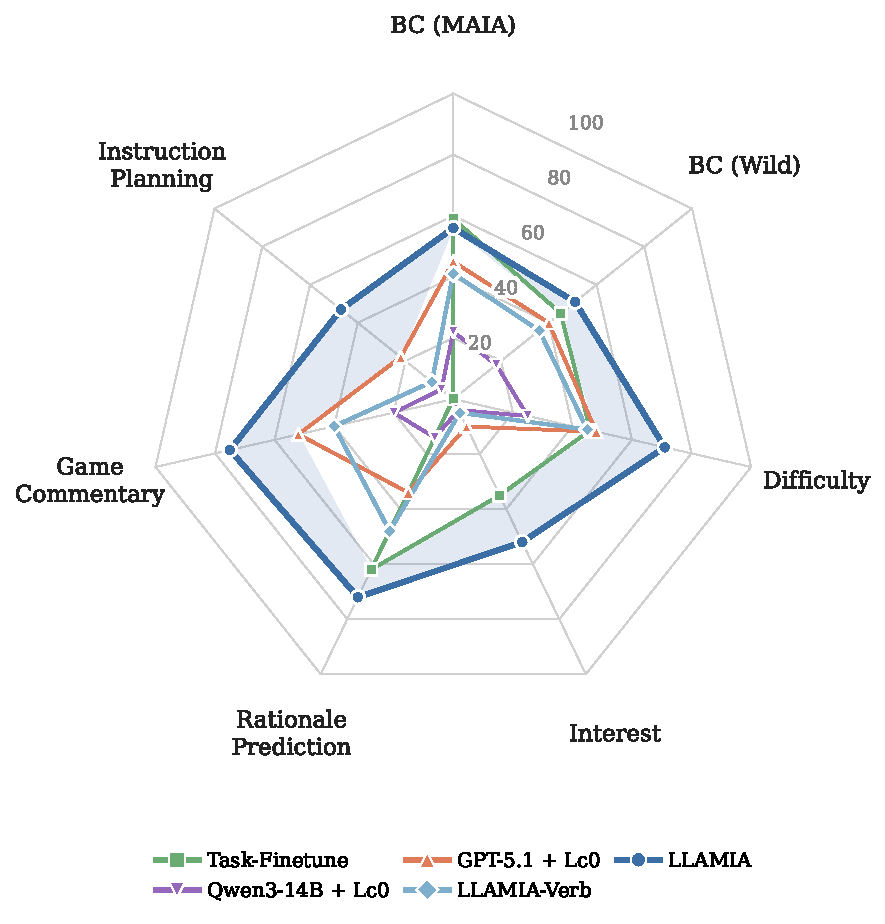
\includegraphics[width=\linewidth]{pages/figures/llamia_bench_radar.pdf}
    \caption{\textbf{LLAMIA-Bench radar: LLAMIA vs.\ LLAMIA-Verb across
    model sizes.}
    Three panels (4B, 8B, 14B) show the verbalization gap at each scale.
    LLAMIA (dark blue, solid) consistently dominates all spokes.
    LLAMIA-Verb (orange, dashed) collapses on Interest
    (non-verbalizable signal) and Instruction Planning (requires
    policy override) at every size. The gap widens with scale on
    multi-step tasks (Commentary, ICP) while remaining roughly
    constant on single-position tasks (BC, Difficulty).
    }
    \label{fig:radar}
\end{figure*}

\begin{figure*}[t]
    \centering
    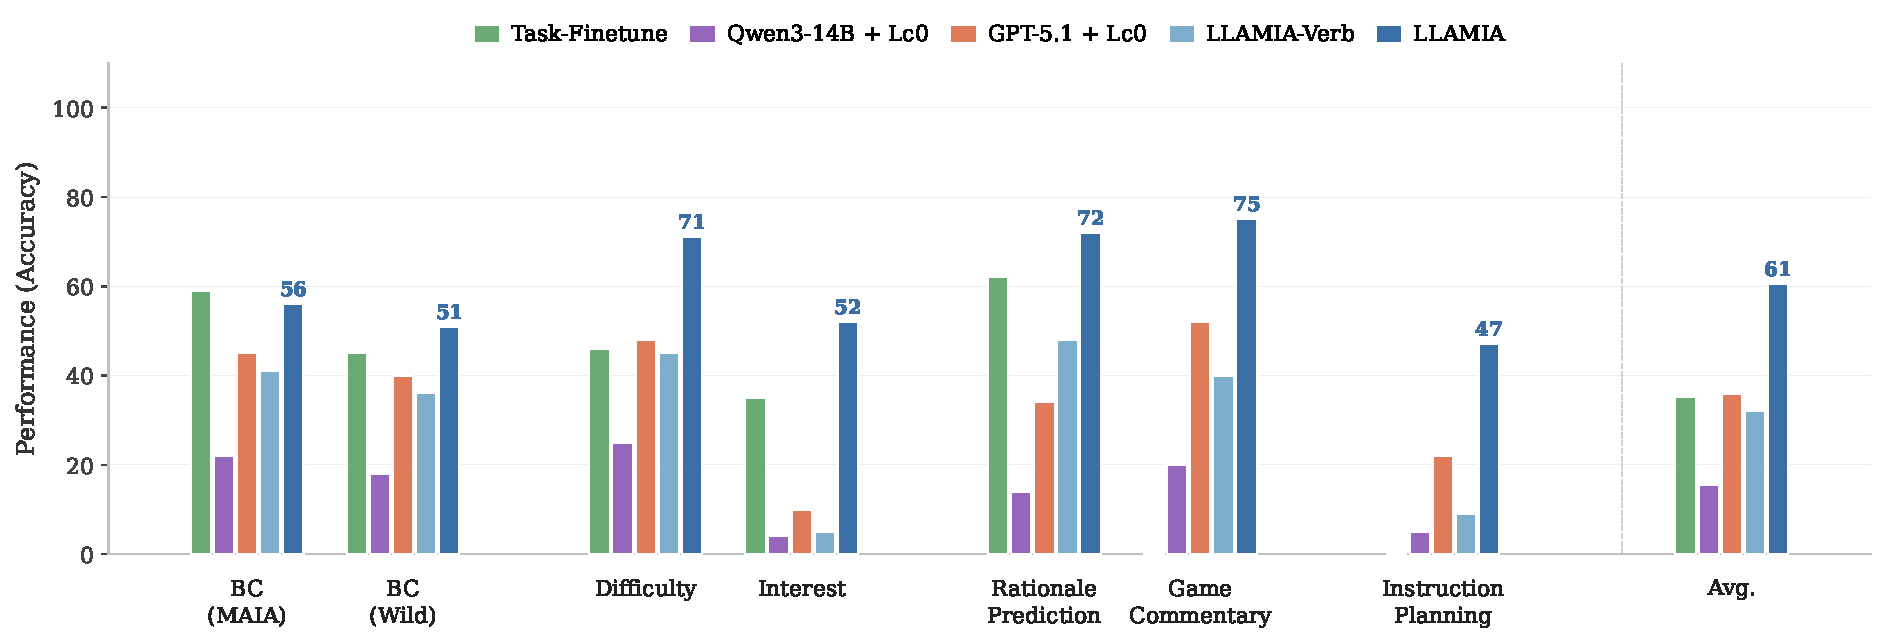
\includegraphics[width=\linewidth]{pages/figures/llamia_bench_bars.pdf}
    \caption{\textbf{LLAMIA-Bench grouped bar chart with improvement arrows.}
    Performance (normalized) across all seven tasks.
    Bars show Task Expert (green, where applicable), Frontier+Tool
    (orange), and LLAMIA at 4B/8B/14B (progressively darker blue).
    Thin arrows indicate relative improvement of each LLAMIA size
    over the matched LLAMIA-Verb baseline.
    Key patterns: (1)~LLAMIA improvement is largest on Interest
    and ICP, confirming the verbalization gap on non-verbalizable
    and multi-step tasks;
    (2)~Task Experts win on in-distribution BC (MAIA) but lose on
    wild splits;
    (3)~no Task Expert exists for Difficulty or Interest prediction.
    }
    \label{fig:bench_bars}
\end{figure*}

\subsection{ICP Eval Reward}
\label{sec:results_icp}

\begin{figure}[t]
    \centering
    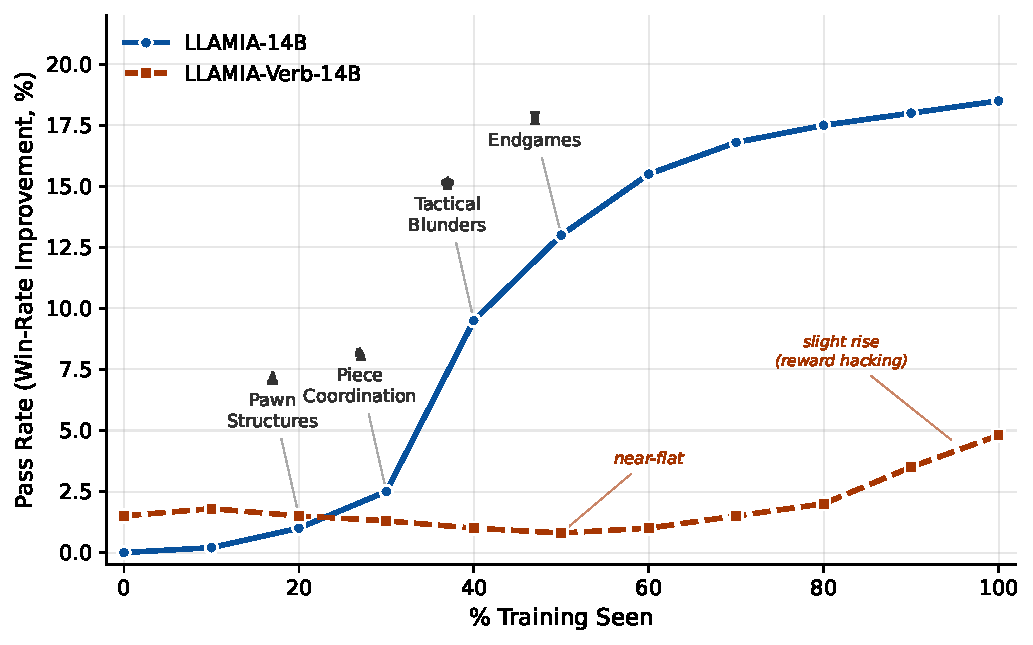
\includegraphics[width=\linewidth]{pages/figures/icp_eval_reward.pdf}
    \caption{\textbf{Instruction-Conditioned Planning: eval reward curve.}
    Pass rate (win-rate improvement, \%) vs.\ \% training seen.
    LLAMIA-14B (blue, solid) acquires motif categories in a
    characteristic order: Pawn Structures and Piece Coordination
    emerge first (${\sim}20$--$30$\%), Tactical Blunders at
    ${\sim}40$\%, Endgames at ${\sim}50$\%.
    Each category shows a sigmoid-like jump.
    LLAMIA-Verb-14B (orange, dashed) remains near-flat throughout
    with minimal improvement even at full data exposure---the slight
    rise at $>90$\% training is consistent with reward hacking
    rather than genuine motif acquisition.
    }
    \label{fig:icp_eval}
\end{figure}
